\documentclass{ctexart}
\usepackage{graphicx}
\usepackage{amsmath}
\usepackage{amsthm}
\usepackage{amssymb}
\usepackage{fancyhdr}
\usepackage{ifthen}
\usepackage{syntonly}
\usepackage[colorlinks, CJKbookmarks=true, linkcolor=red]{hyperref}
\pagestyle{plain}
\usepackage[raggedright]{titlesec}
\newtheorem{性质}{性质}
\newtheorem{定理}{定理}
\newtheorem{推论}{推论}
\begin{document}
\title{《特征提取方法综述》读书报告}
\author{计算机科学与技术系52班 杨定澄 \and 学号:2015011274 \and E-mail:892431401@qq.com}
\date{}
\maketitle
\section{引言}
这篇论文做了一个现有的基于图形的特征提取方法的综述。有效的图形特征提取需要满足一些基本的性质,如:

\begin{itemize}
\item 可辨别性。
\item 平移、旋转、缩放不变性。即平移、旋转、缩放不会影响特征的提取。
\item 仿射不变性。仿射变换是从一个坐标系到另一个坐标系的线性映射,保持二维图形的“平直性”(即变换后直线还是直线不会打弯,圆弧还是圆弧)和“平行性”(其实是指保持二维图形间的相对位置关系不变,平行线还是平行线,而直线上点的位置顺序不变,另特别注意向量间夹角可能会发生变化。)。他可以看做一系列平移、缩放、翻转、旋转和错切的变换进行复合。特征的提取要尽可能不受仿射变换的影响。
\item 抗噪声:特征必须尽量有对噪声的鲁棒性。
\item 掩蔽不变性:当图片的一部分被遮住,剩余部分的特征不变
\item 统计独立性:两个特征需要相互独立。
\item 可靠性:只要处理同一个图像,提取出来的特征就应该是相同的
\end{itemize}

通常,图形的描述是用一组数表示的,或者说是以向量的形式,一般满足如下几个要求:

\begin{itemize}
\item 对信息的描述要尽可能完整
\item 描述要尽可能简洁,这样向量的大小就不会太大。
\item 对两个向量计算“相似程度”(定义为向量距离)的算法不能太复杂,不然运行时间会相当长。
\end{itemize}

图像特征的提取与表示在下列应用中扮演重要角色:

\begin{itemize}
\item 图像搜索:在拥有海量图像的数据库中搜索一张图像,一般是通过计算向量距离选取最小的来实现。
\item 图像的识别与分类:通过对向量进行匹配,按特征向量的相似程度分类。
\item 图像的对齐与校准:通过一些变换使特征向量尽可能相似,从而达到效果。
\item 图像的近似与简化:重新构造一个尽可能相似的图像,满足特征向量比较接近。
\end{itemize}

图像的特征有很多种,他们各具特点。有的容易计算且直观,有的计算时间复杂度低,有的不变性好,有的对于噪声具有优秀的鲁棒性。

我们应该结合他们各自的特征,针对具体问题具体分析。

这篇论文是一篇综述性质的论文,故详略不一的介绍了各种各样的特征提取方法,下图是一张目录。

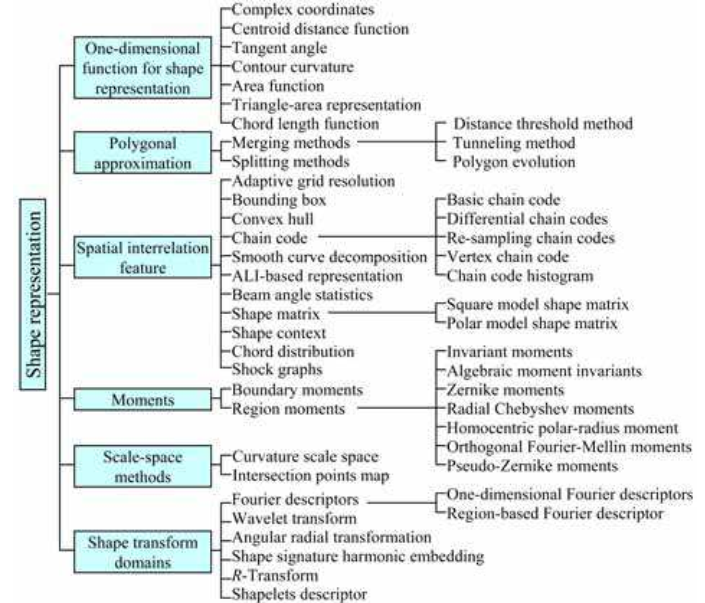
\includegraphics{1.png}

接下来,将会按照目录的顺序进行简单的介绍。

\textbf{由于这篇论文的很多术语找不到比较正式的中文翻译,所以接下来的很多术语我都会注明他的英文。}

\section{形状参数(Shape parameters)}
我们可以用一些图像的参数来表示,包括“Center of gravity, Axis of least inertia, Digital bending energy, Eccentricity, Circularity ratio, Elliptic variance, Rectangularity, Convexity, Solidity, Euler number, Profiles, Hole area ratio”

\subsection{重心(Center of gravity)}
重心也被称为质心(其实并不完全正确),我们假设要处理的二维图形轮廓为区域$D$,定义函数

\[f(x,y)=\begin{cases}1 & if\quad (x,y) \in D \\ 0 & otherwise\end{cases}\]

定义$N$为区域上的点数,即集合$\{(x,y)|f(x,y)=1\}$的大小。那么质心$(g_x,g_y)$就满足:

\[\begin{cases}g_x=\frac{1}{N}\sum\limits_{i=1}^Nx_i \\ g_y=\frac{1}{N}\sum\limits_{i=1}^Ny_i\end{cases}\]

但是直接用这个公式,得到的结果会受具体点的分布疏密程度的影响(因为这是轮廓线重心而不是图形重心)

假设轮廓是闭曲线,记离散参数方程为$\Gamma(n)=(x(n),y(n)),n \in [0,N-1],\Gamma(N)=\Gamma(0)$。

接着介绍一点有关重心的知识。假设要计算一个多边形的重心,一个方法是将多边形分割成若干个部分,算出每一个部分的面积和重心。接着按加权平均就得到整个多边形的重心。而最简单的多边形,自然就是三角形了。

三角形的重心和面积都能非常容易的计算,如果一个三角形的点是$(x_1,y_1),(x_2,y_2),(x_3,y_3)$,那么重心就是$(\frac{x_1+x_2+x_3}{3},\frac{y_1+y_2+y_3}{3})$,而面积可以用叉积计算。

另外,计算一个多边形的面积有这么一个方法,假设多边形是$(P_1,P_2,P_3,\cdots,P_n)$,我们可以拆成恰好$n$个三角形,其中第$i$个三角形是$OP_iP_{i+1}(1 \le i < n)$,而第$n$个三角形是$OP_nP_1$,$O$是坐标轴原点。接着计算他们的\textbf{有向面积}相加,不在多边形内的部分会正负相抵。

重心同样可以用这种方法计算,因此我们可以导出重心公式。

对于三角形$OP_iP_{i+1}$,他的有向面积是$x_iy_{i+1}-y_ix_{i+1}$,重心是$(\frac{x_i+x_{i+1}}{3},\frac{y_i+y_{i+1}}{3})$

首先计算多边形的面积为$A=\frac{1}{2}|\sum\limits_{i=0}^{N-1}(x_iy_{i+1}-x_{i+1}y_i)|$,接着导出多边形重心坐标公式:

\[\begin{cases}g_x =\frac{1}{6A}\sum\limits_{i=0}^{N-1}(x_i+x_{i+1})(x_iy_{i+1}-x_{i+1}y_i) \\ g_y  = \frac{1}{6A}\sum\limits_{i=0}^{N-1}(y_i+y_{i+1})(x_iy_{i+1}-x_{i+1}y_i)\end{cases}\]
\subsection{最小惯性轴(Axis of least inertia)}
仍然用轮廓表示物体。

若一个物体对于某个轴的转动惯量最小,这个轴称为他的最小转动轴。

即对于一个物体,找一个轴,使得轮廓上每个点到这个轴的距离的平方和最小,就是最小转动轴。

最小转动轴同样是一个比较好的用来比较两个图像的参数。

根据物理定义,最小转动轴必定经过重心。我们通过平移变换将重心移到原点,假设最小转动轴的极角为$\theta$,就知道他的参数方程是$x\sin(\theta)-y\cos(\theta)=0$。

定义$a=\sum\limits_{i=0}^{N-1}x_i^2,b=\sum\limits_{i=0}^{N-1}2x_iy_i,c=\sum\limits_{i=0}^{N-1}y_i^2$,定义最小转动轴与$x$轴的夹角为$\alpha$。

我们知道对于直线$Ax+By+C=0$,点$P(x,y)$到直线的距离公式是:

\[\frac{|Ax+By+C|}{\sqrt{A^2+B^2+C^2}}\]

在这个问题中,直线是$x\sin(\theta)-y\cos(\theta)=0$。故有$C=0,A^2+B^2=1$。

代入公式并展开,配合三角函数的二倍角公式,就可以算出惯量为$I=\frac{1}{2}(a+c)-\frac{1}{2}(a-c)\cos(2\alpha)-\frac{1}{2}b\sin(2\alpha)$。

求导可知,$\frac{dI}{d\alpha}=(a-c)\sin(2\alpha)-b\cos(2\alpha),\frac{d^2I}{d\alpha^2}=2(a-c)\cos(2\alpha)+2b\sin(2\alpha)$

令$\frac{dI}{d\alpha}=0$,可解出

\[\alpha=\frac{1}{2}\arctan(\frac{b}{a-c}),-\frac{\pi}{2}<\alpha<\frac{\pi}{2}\]

接着就知道
\[\theta=\begin{cases}\alpha+\frac{\pi}{2} \quad if \frac{d^2I}{d\alpha^2}<0 \\ \alpha \quad otherwise\end{cases}\]
\subsection{平均弯曲能量(Average bending energy)}
定义$BE=\frac{1}{N}\sum\limits_{s=0}^{N-1}K(s)^2$,$K(s)$为曲率函数,$s$是弧长参数,$N$是轮廓线上的点数。

具体计算较为麻烦,论文中也只是引用了别人的工作而没有详细讲解。

可以证明圆是具有最小平均弯曲能量的图形。
\subsection{离心率(Eccentricity)}
离心率的数学定义应该是焦点间距离和长轴的比值,大概是因为这样子不方便计算,论文中将离心率定义为计算长轴与短轴的比值。

离心率可以用主轴法或最小边界矩形法计算。
\subsubsection{主轴法(Principal axes method)}
定义图形的协方差矩阵$C$为:

\[C=\frac{1}{N}\sum_{i=0}^{N-1}\begin{bmatrix}x_i-g_x \\ y_i-g_y\end{bmatrix}\begin{bmatrix}x_i-g_x \\ y_i-g_y\end{bmatrix}^T=\begin{bmatrix}c_{xx} & c_{xy} \\ c_{yx} & c_{yy}\end{bmatrix}\]

接着计算矩阵$C$的特征值,分别为$\lambda_1,\lambda_2,\lambda_1<\lambda_2$,就有离心率为$E=\frac{\lambda_2}{\lambda_1}$
\subsubsection{最小边界矩形法(Minimum bounding rectangle)}

我们用一个最小的矩形来覆盖所有点,假设矩形的长为$L$,宽为$W$,我们就可以通过这个计算了。

在这里提一下如何通过最小的矩形覆盖所有点,如果矩形是横平竖直的话或许很好算,但是考虑到矩形可以旋转(论文中给的例子就是这样的),就不方便计算了。

一个做法是说,我们先对所有点求出凸包,接着可以证明,矩形必有一条边贴着凸包上的某一条边。

枚举这条边,计算对边和临边即可。其中对边一定贴着到他距离最远的点,而临边的计算则可以求出所有点到他的投影,就能得到两个极点,这两个点分别会被两条临别紧贴。

这种方法称之为旋转卡壳法,求出凸包后的复杂度是$O(n)$的。

\subsection{圆率(Circularity ratio)}
他表示一个图形有多接近圆,有$3$种定义:
\begin{itemize}
\item 他的面积与一个拥有同样周长的圆的面积比。$C_1=\frac{A_s}{A_c}$。$A_s$是图形的面积,$A_c$是对应的圆的面积。假设他的周长是$O$,可以算出$A_c=\frac{O^2}{4\pi}$。
\item 由于$4\pi$是常数,我们可以定义第二种圆率为$C_2=\frac{A_s}{O^2}$
\item 定义$d_i=\sqrt{(x_i-g_x)^2+(y_i-g_y)^2}$,$\mu_R=\frac{1}{N}\sum_{i=1}^{N-1}d_i,\sigma_R=\sqrt{\frac{1}{N}\sum_{i=1}^{N-1}(d_i-\mu_R)^2},C_{va}=\frac{\sigma_R}{\mu_R}$
\end{itemize}

\subsection{椭圆方差(Ellipse variance)}
假设$C_e$为主轴法的$C$,再假设

\[V_i=\begin{bmatrix}x_i-g_x \\ y_i-g_y\end{bmatrix}\]

定义$d_i'=\sqrt{V_i^TC_e^{-1}V_i},\mu_R'=\frac{1}{N}\sum\limits_{i=1}^{N-1}d_i',\sigma_R'=\sqrt{\frac{1}{N}\sum\limits_{i=1}^{N-1}(d_i'-\mu_R')^2},E_{va}=\frac{\sigma_R'}{\mu_R'}$
\subsection{矩形度(Rectangularity)}
假设$A_s$为图形的面积,$A_R$为最小外接矩形的面积。

他的矩形度就定义为$\frac{A_s}{A_R}$
\subsection{凸性(Convexity)}
凸性定义为图形的凸包周长与图形的周长的比值。
\subsection{固性(Solidity)}
定义为图形的面积与凸包面积的比值。
\subsection{欧拉数(Euler number)}
欧拉数用来表示一个图形的联通块个数与洞数之差。
\subsection{外形(Profiles)}
用来表示投影到$x$轴和投影到$y$轴的信息。

$pro_x(i)=\sum\limits_{j=jmin}^{jmax}f(i,j),pro_y(j)=\sum\limits_{i=imin}^{imax}f(i,j)$

$f(x,y)$的定义和重心时的定义一样。

\subsection{洞面比(Hole area ratio)}

假设$A_s$表示面积,$A_h$表示所有洞的面积,$HAR=\frac{A_h}{A_s}$
\section{一维函数表示法(One-dimensional function for shape representation)}
上面的方法都是通过图形的某个参数来表示,接着我们考虑计算一个图形的某个函数。

\subsection{复数坐标(Complex coordinates)}
对于轮廓线上的点$P_n(x(n),y(n))$,记$z(n)=[x(n)-g_x]+i[y(n)-g_y]$

\subsection{质心距离函数(Centroid distance function)}
定义$r(n)=[(x(n)-g_x)^2+(y(n)-g_y)^2]$

\subsection{正切角(Tangent angle)}

定义$\theta(n)=\theta_n=\arctan(\frac{y(n)-y(n-w)}{x(n)-x(n-w)})$,$w$自己定。

该方法对噪声是比较敏感的,所以一般要先进行过滤。此外,该方法得到的$\theta(n)$将不连续,我们可以定义$\varphi(n)=[\theta(n)-\theta(0)],t=\frac{2\pi n}{N}$,就有$\varphi(n)=\varphi(\frac{tN}{2\pi})$,最后定义$\psi(t)=\varphi(\frac{tN}{2\pi})-t,t \in [0,2\pi]$,这样就好些了。

\subsection{轮廓曲率( Contour curvature)}
曲率函数:$K(n)=\frac{x'(n)y''(n)-y'(n)x''(n)}{(x'(n)^2+y'(n)^2)^{3/2}}$。

假设改为弧长参数方程,即$x=x(s),y=y(s)$,矢函数$r(s)=(x(s),y(s))$,就有$K(s)=\frac{x'(s)y''(s)-y'(s)x''(s))}{r'(s)^3}$。

\textbf{曲线以弧长为参数时,其切矢量为单位矢量}

因此就有$K(s)=x'(s)y''(s)-y'(s)x''(s)$

该参数在平移、旋转操作下不会有影响,但是在缩放操作下会成比例的变化。为了处理这种现象,我们令$K'(s)=\frac{K(s)}{\frac{1}{N}\sum_{s=1}^N|K(s)|}$

对于弧长的计算,可以用向心法近似:

定义$d_n$为点$P_n$与$P_{n+1}$的距离,$P=\sum\limits_{n=1}^Nd_n,L=\sum\limits_{n=1}^N\sqrt{d_n}$,令$s_1=0,s_k=s_{k-1}+\frac{P\sqrt{d_{k-1}}}{L}$。

\subsection{面积函数(Area function)}

定义$S(n)$表示点$P_n,P_{n+1},(g_x,g_y)$所构成的三角形面积。

\subsection{三角面积表示(Triangle-area representation)}

自己拟定一个$t_s$,记$TAR(n,t_s)$为$\Delta P_{n-t_s}P_nP_{n+t_s}$的有向面积,即

\[TAR(n,t_s)=\frac{1}{2} \begin{vmatrix}x_{n-t_s} & y_{n-t_s} & 1\\x_n & y_n & 1 \\x_{n+t_s} & y_{n+t_s} & 1\end{vmatrix}\]

\subsection{弦长函数(Chord length function)}

对于点$P$,过他作法向量,取轮廓线上最近的交点$P'$,从而得到$PP'$间距离。这个量在平移后不会变,但对噪声比较敏感。

\section{多边形近似(Polygonal approximation)}
多边形近似指的是通过一个多边形来近似给定的轮廓线,主要操作分为合并和分裂两部分。
\subsection{合并(Merging methods)}
\subsubsection{距离阈值法(Distance threshold method)}

我们枚举每个像素点,一个个加入。一开始先选择一个点作起始点。

当新添加一个像素点时,做一条直线连接他和起始点,然后计算他们之间的点中和直线距离的最值,拿他和阈值进行比较。

如果超过了阈值,就改为一条线段从起始点直接连到他的上一个点再连到他。

对于点$P_i(x_i,y_i),P_j(x_j,y_j),P_k(x_k,y_k)$,可以算出点$P_k$到直线$P_iP_j$的最近距离为:

\[d_k(i,j)=\frac{|(x_j-x_i)(y_i-y_k)-(x_i-x_k)(y_j-y_i)|}{\sqrt{(x_j-x_i)^2+(y_j-y_i)^2}}\]

\subsubsection{隧道法(Tunneling method)}

我们试着用一条隧道来近似轮廓线,隧道由一些直线段组成,但要尽可能地减少线段个数。

我们任取一个点从他出发,沿着轮廓线建立隧道,直到曲率过大以至于无法继续走时,新建一个隧道来转弯。

这样子一直走到终点,就叫隧道法。
\subsubsection{多边形变换(Polygon evolution)}

多边形变换的思路很简单,每一步变换操作,选择相邻的两条直线段,试着将他们合并成一条。

假设线段分别是$s_1,s_2$,定义$\beta(s_1,s_2)$为两线段的夹角,而$l(s)$为线段$s$的长度。

定义$K(s_1,s_2)=\frac{\beta(s_1,s_2)l(s_1)l(s_2)}{l(s_1)+l(s_2)}$

那么当$K(s_1,s_2)$足够小时,就意味着这两条线段并不重要,可以合并为一条了。
\subsection{分裂}

分裂操作是当多边形的近似程度不令人满意时,进一步逼近的手段。他是合并的逆过程。

对于多边形上的一条边$AB$,考虑轮廓线上$AB$间的每个点,计算这些点到$AB$的距离,选出最远点$P$。

如果$P$到$AB$的距离过于大了,就将边$AB$分裂为$AP$和$PB$。
\section{空间关系特征(Spatial interrelation feature)}
\subsection{自适应网格分辨率(Adaptive grid resolution)}
首先要介绍一下四分树的概念。

四分树是一个数据结构,可以看做一维线段树在二维平面上的自然扩展。

这个数据结构是一棵四叉树,对于树上每一个点,会代表一个正方形区域。接着,将这个正方形一分为四,就能作为他的四个儿子。

我们从根节点出发递归建树,假设对应区域全是$1$,就停下来;如果不全是$1$,就一分为四递归建立。

很显然得到的四分树,对于旋转操作不具有不变性。为此我们可以在一开始,就按照某个要求将图形先旋转成某个标准形式,这样的话就能保证旋转不变性了。

至于这个标准形式是什么呢?我们先找到距离最远的两个点$P_1,P_2$,然后将他们旋转使得$P_1P_2$平行于$x$轴。可是即使如此仍然有两种可能(即$P_1$在左边还是右边),我们再严格要求质心在$P_1P_2$下方,这样就只有一种标准形式了。

这么一来,就具有旋转不变性。同时,由于$P_1,P_2$是相隔最远的两个点,我们就可以做一个边长为$P_1P_2$的正方形,包含所有点了。这个正方形正好可以用作四分树根节点所对应的正方形。

从根节点出发,递归建立四分树。

这么一来,首先他在平移、旋转下得到的四分树肯定是一样的,对于缩放操作,由于根节点所对应会跟着缩放,所以仍然是不变的。

因此,它具有自适应的特点。

\subsection{边界框(Bounding box)}
首先和上面的方法一样,仍然是要旋转到标准形式保持不变性。

接着构造一个边长平行于坐标轴的$w \times h$的矩形将图形覆盖,然后人为定义参数$n,m$,将它分成$n \times m$个部分。

注意并不是均匀地分成这么多部分,而是先将矩形的长边均匀分成$n$份,对于每一份,找到该区域里的点的纵坐标的最小最大值,从而得到包含这一部分点的矩形高度,再均匀分成$m$份。

这样的好处是他是自适应的。

最后具体到表示法,假设$(v_x,v_y)$是最开始的覆盖所有点的矩形的左下角左边,$B_{ij}$是第$i$行$j$列个小矩形,他的中心坐标是$(u_x^{ij},u_y^{ij})$,就定义
\[\begin{bmatrix}\mu_x^{ij} \\ \mu_y^{ij}\end{bmatrix}=\begin{bmatrix}(\mu_x^{ij}-v_x)/w \\ (\mu_y^{ij}-v_y)/h\end{bmatrix}\]
\subsection{凸包法(Convex hull)}
凸包指的是用一个最小的凸多边形保住所有的点。

凸包的求法有很多,这里为了方便表示,使用一种叫concavity tree的数据结构递归求凸包,而求解过程得到的信息就能用来表示了。

而他也是在平移、旋转、缩放下不变的一个量,并对噪声有较强的鲁棒性。(大多数噪音点是不会对凸包产生影响的)
\subsection{链码(Chain code)}
链码是用来描述轮廓线的。
\subsubsection{基本链码(Basic chain code)}
一个轮廓线可以看做是四联通或者八连通的,我们沿着轮廓线运动的过程可以看做是一个方向集合,方向集合用$\{i|i=0,1,\cdots,7\}$或$\{i|0,1,2,3\}$表示。

这种表示法在平移下是不变的,我们可以进行一些处理使得他在旋转下也不变。

一个技巧叫Differential chain codes,意思就是对得到的方向向量在模意义下做差分。
\subsubsection{顶点链码(Vertex chain code)}
我们只考虑轮廓线上的点,把点分成$3$类:
\begin{enumerate}
\item 边上的点,记作$2$
\item 如果是角落上的点,角度为$90\circ$,记作$1$
\item 如果是角落上的点,角度是$270\circ$,记作$2$
\end{enumerate}•

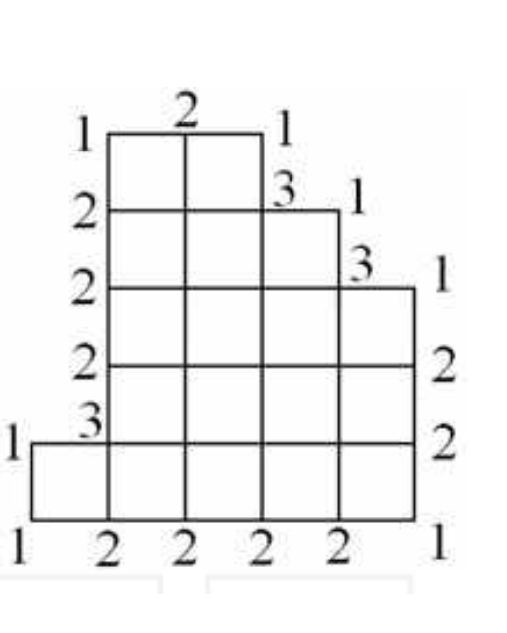
\includegraphics{2.png}

这里有一个清楚的例子。
\subsubsection{链码直方图}
将得到的链码画出一张直方图。
\subsection{平滑曲线分解(Smooth curve decomposition)}
将轮廓线分解成若干段高斯平滑曲线。

对每一段曲线,记录他的两个属性。第一个是这段曲线里的曲率函数最大值,另一个则是曲线的方向。
\subsection{基于最小惯性轴的符号表示(Symbolic representation based on the axis of least inertia)}
我们求出最小惯性轴后,将图像上的点在轴上做投影,就能在最小惯性轴上得到许多点,其中有两个极点。

连接他们得到一条线段,将这条线段$n$等分,就能等间距地取到若干特征点。

对于每一个特征点,做垂直于最小惯性轴的垂线,就能与图像产生若干个交点,得到若干段在图像内的线段。

将这些线段的长度排好序,就得到集合$f_i$,最后将集合全部考虑进来就有特征向量$F=[f_1,f_2,\cdots,f_n]$
\subsection{光束角度统计(Beam angle statistics)}
对于第$i$个点,定义$C_k(i)=\theta_{V_{i+k}}-\theta_{V_{i-k}}$,而$\theta_{V_{i+k}}=\arctan\frac{y_{i+k}-y_i}{x_{i+k}-x_i},\theta_{V_{i-k}}=\arctan\frac{y_{i-k}-y_i}{x_{i-k}-x_i}$。

最后求$C_k^m(i)$的期望,即$\sum\limits_{k=1}^{N/2-1}C_k^m(i)P_k(C_k(i))$
\subsection{图像矩阵(Shape matrix)}
\subsubsection{方形模型图像矩阵(Square model shape matrix)}
先求出图形的质心$G$,求出图形中到质心最远的点,假设距离为$L$。

以质心为中心,做一个边长为$2L$的、包含整个图形的正方形,将它平均分成$n \times n$个小格子。

定义$\mu(S)$表示图形$S$的面积,$S$表示整个图形,$S_{kj}$表示第$k$行$j$列个小格子,就能定义出矩阵$B$:

\[B_{kj}=\begin{cases}
1 & \mu(S_{kj}\cap S) \ge \mu(S_{kj})/2 \\ 0 & otherwise
\end{cases}\]
\subsubsection{极角模型图像矩阵(Polar model shape matrix)}
和方形模型类似,只不过是按$\theta,r$这两个量均匀分成$n \times m$个部分。

最后得到一个$n \times m$的矩阵。
\subsubsection{图像文本(Shape context)}
现在图像里采样若干个点。

对于一个采样点,以他为中心建立极角坐标系,将极角坐标系按纬度和距离分成若干段,对每一段内的点数进行统计。

这种方法依据和其他点的相关关系,从而能比较像素点的相似程度。

采样点越多,方法月精准。
\subsubsection{弦分布(Chord distribution)}
统计每对点的距离,可以看做是统计每条弦长。

对得到的统计结果建立直方图。
\subsubsection{震动图(Shock graphs)}
这个方法可以看做是求出一个图的“骨架”。

每次在中心做一个和图形双切的圆,分成两部分分治做下去。

最后中心的移动轨迹就成了一个“中轴”。

移动轨迹如果看做是有向的,我们从第一个点出发,就能得到一张有向无环图了。
\section{矩}
\subsection{边界矩(Boundary moments)}
我们先来定义$r$阶矩和$r$阶中心矩:

\[m_r=\frac{1}{N}\sum_{i=1}^N[z(i)]^r,\mu_r=\frac{1}{N}\sum_{i=1}^N[z(i)-m_1]^r\]

根据定义,我们可以对轮廓线求矩。矩的计算并不难,但他要计算$r$次方,可能导致值过大。
\subsection{区域矩(Region moments)}
顾名思义,上面是对轮廓线求矩,这里就改成对区域求矩了。

\[m_{pq}=\sum_x\sum_y\Psi_{pq}(x,y)f(x,y)\]

$\Psi$函数是自己定义的。
\subsubsection{不变矩(Invariant moments)}
我们定义$\Psi_{pq}(x,y)=x^py^q$,代入上式得到几何矩:

\[m_{pq}=\sum_x\sum_yx^py^qf(x,y)\]

再定义中心矩

\[\mu_{pq}=\sum_x\sum_y(x-\bar{x})^p(y-\bar{y})^qf(x,y)\]

一些比较好的矩不受平移、旋转和缩放、镜面变换的影响,他们包括

\begin{align*}
& \phi_1=\eta_{20}+\eta_{02} \\
& \phi_2=(\eta_{20}-\eta_{02})^2+4\eta_{11}^2 \\
& \phi_3=(\eta_{30}-3\eta_{12})^2+(3\eta_{21}-\eta_{03})^2 \\
& \phi_4=(\eta_{30}+\eta_{12})^2+(\eta_{21}+\eta_{03})^2 \\
& \phi_5=(\eta_{30}-3\eta_{12})(\eta_{30}+\eta_{12})[(\eta_{30}+\eta_{12})^2-3(\eta_{21}+\eta_{03})^2] \\
& +(3\eta_{21}-\eta_{03})(\eta_{21}+\eta_{03})[3(\eta_{30}+\eta_{12})^2-(\eta_{21}+\eta_{03})^2] \\
& \phi_6=(\eta_{20}-\eta_{02})[(\eta_{30}+\eta_{12})^2-(\eta_{21}+\eta_{03})^2] \\ 
& +4\eta_{11}(\eta_{30}+\eta_{12})(\eta_{21}+\eta_{03}) \\
& \phi_7=(3\eta_{21}-\eta_{02})(\eta_{30}+\eta_{12})[(\eta_{30}+\eta_{12})^2-3(\eta_{21}+\eta_{03})^2] \\
& +(3\eta_{12}-\eta_{30})(\eta_{21}+\eta_{03})[3(\eta_{30}+\eta_{12})^2-(\eta_{21}+\eta_{03})^2]
\end{align*}

这种做法一个缺点是涉及到指数函数,会导致值过大。
\subsubsection{代数不变矩(Algebraic moment invariants)}
将前$k$阶中心矩,作为一个矩阵的特征值。
\subsubsection{Zernike矩(Zernike moments)}
Zernike曾提出一组在单位圆上的正交多项式,定义为:
\[V_{nm}(x,y)=V_{nm}(r \cos \theta,r \sin \theta)=R_{nm}(r)\exp(jm\theta) \]

\[R_{nm}(r)=\sum_{s=0}^{n-|m|/2}(-1)^s\frac{(n-s)!}{s! \times (\frac{n-2s+|m|}{2})!(\frac{n-2s-|m|}{2})!}r^{n-2s}\]

然后定义Zernike矩:

\[Z_{nm}=\frac{n+1}{\pi}\sum_r\sum_{\theta}f(r\cos \theta,r \sin \theta)R_{nm}(r)\exp(jm\theta)\]
\subsubsection{径向切比雪夫矩(Radial Chebyshev moments)}
定义径向切比雪夫矩:

\[S_{pq}=\frac{1}{2\pi \rho(p,m)}\sum_{r=0}^{m-1}\sum_{\theta=0}^{2\pi}t_p(r)\exp(-jq\theta)f(r,\theta)\]

其中$t_p(r)$的定义是:

\begin{align*}
& t_0(x)=1 \\
& t_1(x)=(2x-N+1)/N \\
& t_p(x)=\frac{(2p-1)t_1(x)t_{p-1}(x)-(p-1)(1-\frac{(p-1)^2}{N^2})t_{p-2}(x)}{p}
\end{align*}

$\rho(p,N)$的定义是:

\[\rho(p,N)=\frac{N(1-\frac{1}{N^2})(1-\frac{2^2}{N^2})\cdots (1-\frac{p^2}{N^2})}{2p+1},m=1+\frac{N}{2}\]

$(r,\theta)$与$(x,y)$的映射关系是:

\begin{align*}
& x=\frac{rN}{2(m-1)}\cos(\theta)+\frac{N}{2} \\
& y=\frac{rN}{2(m-1)}\sin(\theta)+\frac{N}{2}
\end{align*}
\section{尺度空间方法(Scale space approaches)}
\subsection{曲率尺度空间(Curvature scale-space)}
将曲线用参数$\mu$表示$\Gamma(\mu)=(x(\mu),y(\mu)),\Gamma_{\sigma}(\mu)=(X(\mu,\sigma),Y(\mu,\sigma))$

定义$*$为卷积,有$X(\mu,\sigma)=x(\mu)*g(\mu,\sigma),Y(\mu,\sigma)=y(\mu)*g(\mu,\sigma)$,而$g$函数则是正态分布的密度函数:

\[g(\mu,\sigma)=\frac{1}{\sqrt{2 \pi \sigma^2}} \exp(-\frac{\mu^2}{2\sigma^2})\]

有了函数$X,Y$后,就能求出关于$\mu$的曲率,以及$X,Y$各自关于$\mu$的一阶、二阶导。
\subsection{交叉点地图(Intersection points map)}
还可以用一个高斯平滑曲线来近似,并通过新曲线与原曲线的交点信息代替二阶导。
\section{图像变换域(Shape transform domains)}
\subsection{傅里叶描述子(Fourier Descriptor)}
\subsubsection{一维傅里叶描述子(One-dimensional Fourier descriptors)}
对于每个点$t$计算出质心距离函数$r(t)$,再通过质心距离函数得到傅里叶系数

\[a_n=\frac{1}{N}\sum_{t=0}^{N-1}r(t)\exp(\frac{-j2\pi nt}{N}),n=0,1,\cdots,N-1\]

显然,对于平移、旋转,得到的傅里叶系数都保持不变。对于缩放操作,以及把起点从初始点变为另一个点,初始系数是$a_n^{(o)}$。假设$s$为缩放因子,$\tau$表示初始点下标变化量,可计算新的傅里叶系数
\[a_n=\exp(jn\tau) \times s \times a_n^{(o)}\]

记$b_n=\frac{a_n}{a_1}$,可以发现有$|b_n|=|b_n^{(o)}|$,也就是说$|b_n|$是对平移、旋转、缩放、换一个初始点都不变的量。
\subsubsection{基于区域的傅里叶描述子(Region-based Fourier descriptor)}
首先要将极坐标系转为笛卡尔坐标系,步骤如下:

\begin{enumerate}
\item 将图像旋转一个角度。
\item 沿$x$轴正方向将像素点拷贝
\item 不断重复,直到转过360$^\circ$
\end{enumerate}

这么一来,就实现了极坐标系和笛卡尔坐标系的转化。定义函数$f(r, \theta_i)$类似于求质心时的$f(x,y)$,来求函数$pf$:

\[pf(\rho,\phi)=\sum_r\sum_if(r,\theta_i)\exp[j2\pi(\frac{r}{R}\rho+\frac{2\pi i}{T}\phi)]\]

最后用$GFD$来描述区域,假设$S$代表面积,$GFD$定义为:

\[GFD=\{\frac{|pf(0,0)|}{S},|\frac{pf(0,1)}{pf(0,0)}|,\cdots,|\frac{pf(0,n)}{pf(0,0)}|,\cdots,|\frac{pf(m,0)}{pf(0,0)}|,\cdots,|\frac{pf(m,n)}{pf(0,0)}|\}\]

\subsection{小波变换(Wavelet transform)}
小波变换是继承自傅里叶变换的另外一种变换分析方法,有不少优秀的性质,应用非常广泛。
\subsection{角径向变换(Angular radial transformation)}
定义
\[A_m(\theta)=\frac{1}{2\pi}e^{jm\theta}\]
\[R_n(\rho)=\begin{cases}1 & n=0 \\ 2\cos(n\rho \pi) & n \neq 0\end{cases}\]
\[V_{nm}(\rho,\theta)=A_m(\theta)R_n(\rho)\]
\[F_{nm}=\int_0^{2\pi}\int_0^1V_{nm}(\rho,\theta)f(\rho,\theta)\rho d \rho d \theta\]

随着$n,m$的不同取值,将得到不同的结果。这种表示法在平移、缩放下都是鲁棒的。
\subsection{图像特征谐波嵌入(Shape signature harmonic embedding)}
定义泊松核函数

\[P_R(r,\theta)=\frac{R^2-r^2}{R^2-2Rr\cos(\theta)+r^2}\]

对于任何一种图像特征$s[n],n=0,1,\cdots,N-1$,我们定义$u(Re^{j\phi})=u(Re^{j\omega_0n})=s[n]$,其中$\omega_0=\frac{2\pi}{N},\phi=\omega_0n$

谐波函数$u$就能写作

\[u(re^{j\theta})=\frac{1}{2\pi}\int_0^{2\pi}u(Re^{j\phi})P_R(r,\phi-\theta)d\phi\]

\subsection{R-变换(R-Transform)}
在原论文中不是$R$,而是一个奇怪的字符,不会打。

首先定义Radon变换为
\[T_R(\rho,\theta)=\int_{-\infty}^{\infty}\int_{-\infty}^{\infty}f(x,y)\delta(x\cos(\theta)+y\sin(\theta)-\rho)dxdy\]
\[\delta(x)=\begin{cases}1 & x=0 \\ 0 & otherwise\end{cases}\]

该变换本质是在直线$\rho=x\cos(\theta)+y\sin(\theta)$上进行积分。

接着再定义R变换

\[R_f(\theta)=\int_{-\infty}^{\infty}T_R^2(\rho,\theta)d\rho\]

该变换还能和傅里叶变换相结合,得到一种新的表示法$RTD$。
\section{总结}
阅读这篇论文带给了我很大的收获。

这篇论文主要的思想就是通过各种各样的方式寻找一个图形各种各样的量,这些量可以是一个值,可以是一个函数,可以是一个矩阵。

通过比较量的距离,来比较图像的相似程度。

而不同的量有不同的优势,可以针对不同的变换方法。

有的量比较容易,比如质心,最小惯性轴;但有的量需要用到相对较为高深的数学知识,如最后两章。
\end{document}
